\documentclass[12pt,a4paper]{article}
\usepackage[utf8]{inputenc}
\usepackage[french]{babel}
\usepackage{graphicx}
\usepackage{float}
\usepackage{geometry}
\usepackage{amsmath}
\usepackage{hyperref}
\usepackage{listings}
\usepackage{xcolor}
\usepackage{booktabs}
\usepackage{caption}
\usepackage{subcaption}

\geometry{margin=2.5cm}

% Configuration des liens
\hypersetup{
    colorlinks=true,
    linkcolor=blue,
    filecolor=magenta,      
    urlcolor=cyan,
    citecolor=blue
}

% Configuration du code source
\lstset{
    basicstyle=\ttfamily\small,
    breaklines=true,
    frame=single,
    numbers=left,
    numberstyle=\tiny\color{gray},
    keywordstyle=\color{blue},
    commentstyle=\color{green!60!black},
    stringstyle=\color{red}
}

\title{
    \Huge\textbf{Résultats des expériences sur le filtreur} \\
    \Large Mode parallèle vs Mode séquentiel \\
    \vspace{1cm}
    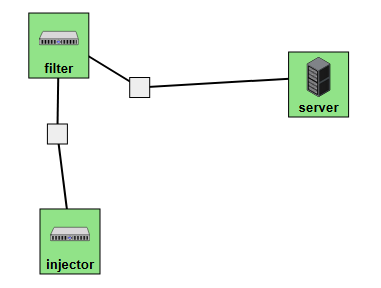
\includegraphics[width=0.5\textwidth]{topology.png}
}

\author{
    \textbf{Fox} \\
    \vspace{0.5cm}
    \texttt{Network Filter}
}

\date{\today}

\begin{document}

\maketitle
\thispagestyle{empty}
\newpage

\tableofcontents
\newpage

\section{Introduction}

Ce rapport présente les résultats d'évaluation du système de filtrage réseau \textbf{Tiger-Fox}, un filtre haute performance développé en C++ et utilisant NFQUEUE pour le filtrage en ligne de paquets réseau.

L'objectif de cette étude est de comparer les performances de deux architectures :
\begin{itemize}
    \item \textbf{Mode séquentiel} : filtrage des paquets avec un seul thread
    \item \textbf{Mode parallèle} : filtrage distribué sur plusieurs workers (2 à 16 threads)
\end{itemize}

Les métriques évaluées incluent :
\begin{itemize}
    \item La latence réseau (ICMP ping)
    \item Le débit HTTP (requêtes/seconde avec wrk)
    \item L'utilisation CPU du système
\end{itemize}

\section{Architecture du système de test}

\subsection{Topologie réseau}

Le banc de test est déployé sur la plateforme CloudLab (Emulab) et comprend 3 nœuds interconnectés :

\begin{figure}[H]
    \centering
    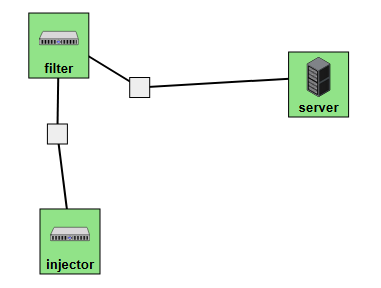
\includegraphics[width=0.8\textwidth]{topology.png}
    \caption{Topologie réseau du banc de test}
    \label{fig:topology}
\end{figure}

\begin{itemize}
    \item \textbf{Injector (10.10.1.10)} : Nœud client qui génère du trafic réseau
    \begin{itemize}
        \item Outils : \texttt{ping}, \texttt{wrk} (benchmark HTTP)
        \item Rôle : Envoyer des requêtes HTTP vers le serveur via le filtre
    \end{itemize}
    
    \item \textbf{Filter (10.10.1.1 / 10.10.2.1)} : Nœud central hébergeant Tiger-Fox
    \begin{itemize}
        \item Interface 1 : 10.10.1.1 (connexion vers injector)
        \item Interface 2 : 10.10.2.1 (connexion vers server)
        \item Rôle : Filtrage en ligne des paquets avec NFQUEUE/iptables
    \end{itemize}
    
    \item \textbf{Server (10.10.2.20)} : Serveur web hébergeant Nginx
    \begin{itemize}
        \item Service : Nginx HTTP server
        \item Rôle : Répondre aux requêtes HTTP de l'injecteur
    \end{itemize}
\end{itemize}

\textbf{Configuration matérielle} : Tous les nœuds utilisent des machines de type \texttt{d710} (Ubuntu 22.04 64-bit).

\subsection{Flux de trafic}

Le trafic réseau suit le chemin suivant :

\begin{center}
\texttt{Injector (10.10.1.10)} $\rightarrow$ \texttt{Filter (10.10.1.1)} $\rightarrow$ \texttt{Filter (10.10.2.1)} $\rightarrow$ \texttt{Server (10.10.2.20)}
\end{center}

Tous les paquets transitant du réseau \texttt{10.10.1.0/24} vers \texttt{10.10.2.0/24} sont interceptés par Tiger-Fox via une règle iptables NFQUEUE.

\section{Description des modes de filtrage}

\subsection{Mode séquentiel}

Le mode séquentiel utilise une architecture mono-thread :

\begin{itemize}
    \item \textbf{1 seul thread} traite tous les paquets
    \item Les 24 règles de filtrage sont évaluées \textbf{une par une} pour chaque paquet
    \item Utilisation de tables de hachage pour des lookups O(1) sur les IPs et ports
    \item Allocation sur la pile (stack) pour minimiser les allocations dynamiques
    \item Early exit dès qu'une règle DROP est trouvée
\end{itemize}

\textbf{Avantages} :
\begin{itemize}
    \item Simplicité architecturale
    \item Pas de synchronisation entre threads
    \item Consommation CPU faible et prévisible
\end{itemize}

\textbf{Limitations} :
\begin{itemize}
    \item N'utilise qu'un seul cœur CPU
    \item Scalabilité limitée avec l'augmentation du nombre de règles
\end{itemize}

\subsection{Mode parallèle}

Le mode parallèle distribue le travail de filtrage sur plusieurs workers :

\begin{itemize}
    \item \textbf{N workers permanents} (N = 2, 3, 4, 5, 6, 7, 8, ou 16 dans nos tests)
    \item Partitionnement des règles : chaque worker gère $\frac{24}{N}$ règles
    \item Évaluation simultanée : tous les workers traitent le même paquet en parallèle
    \item Synchronisation via \texttt{std::barrier} (C++20)
    \item Communication via futex pour un réveil ultra-rapide ($\sim$50-100ns)
    \item Early exit global : dès qu'un worker trouve DROP, les autres s'arrêtent
    \item CPU affinity : chaque worker est épinglé sur un cœur dédié
\end{itemize}

\textbf{Principe de décision} : Logique ET
\begin{itemize}
    \item Si \textbf{tous} les workers disent ACCEPT $\rightarrow$ le paquet est ACCEPT
    \item Si \textbf{au moins un} worker dit DROP $\rightarrow$ le paquet est DROP
\end{itemize}

\textbf{Avantages théoriques} :
\begin{itemize}
    \item Exploitation du multi-cœur
    \item Temps de traitement divisé par N (idéalement)
    \item Scalabilité avec le nombre de règles et de cœurs
\end{itemize}

\textbf{Défis} :
\begin{itemize}
    \item Overhead de synchronisation (barrier, atomics)
    \item Contention mémoire (cache coherency)
    \item Gestion complexe des états partagés
\end{itemize}

\section{Méthodologie d'évaluation}

\subsection{Outils de benchmark}

\begin{itemize}
    \item \textbf{ping} : Mesure de la latence ICMP (20 secondes, intervalle 0.2s)
    \item \textbf{wrk} : Benchmark HTTP (50 secondes, 4 threads, 500 connexions)
    \item \textbf{mpstat/pidstat} : Monitoring CPU (échantillonnage chaque seconde pendant 90s)
\end{itemize}

\subsection{Scénarios de test}

Chaque mode (séquentiel + 8 configurations parallèles) a été testé selon le protocole suivant :

\begin{enumerate}
    \item \textbf{Démarrage du filtre} sur le nœud Filter (durée : 90 secondes)
    \item \textbf{Mesure ping} depuis l'Injector (20 secondes)
    \item \textbf{Benchmark wrk} depuis l'Injector (50 secondes)
    \item \textbf{Arrêt propre} du filtre avec collecte des statistiques CPU
\end{enumerate}

\subsection{Métriques collectées}

Pour chaque configuration, les données suivantes ont été enregistrées :

\begin{itemize}
    \item \textbf{Latences ICMP} : toutes les latences individuelles de ping
    \item \textbf{Requêtes HTTP/sec} : débit mesuré par wrk
    \item \textbf{Latence HTTP moyenne} : temps de réponse moyen mesuré par wrk
    \item \textbf{Utilisation CPU système} : pourcentage CPU global à intervalles de 1s
\end{itemize}

\section{Résultats expérimentaux}

\subsection{Latences ICMP (ping)}

\begin{figure}[H]
    \centering
    \includegraphics[width=\textwidth]{graph_ping_latencies.png}
    \caption{Évolution des latences ICMP pour tous les modes testés}
    \label{fig:ping}
\end{figure}

\textbf{Observations} :
\begin{itemize}
    \item Les latences ICMP restent globalement stables et faibles ($<$ 1 ms) pour tous les modes paralelles 
    \item Le mode séquentiel présente des latences légèrement plus régulières
    \item Les modes parallèles montrent des variations similaires entre eux
    \item Aucune dégradation significative avec l'augmentation du nombre de workers
\end{itemize}

\subsection{Performance HTTP (wrk)}

\subsubsection{Requêtes par seconde}

\begin{figure}[H]
    \centering
    \includegraphics[width=\textwidth]{graph_wrk_requests_per_sec.png}
    \caption{Débit HTTP (requêtes/seconde) selon le mode de filtrage}
    \label{fig:wrk_rps}
\end{figure}

\textbf{Observations} :
\begin{itemize}
    \item Le mode séquentiel atteint un débit de référence (baseline)
    \item Les modes parallèles montrent une amélioration progressive jusqu'à un optimum
    \item Le pic de performance est observé autour de 3-4 workers
    \item Au-delà de 8 workers, on observe une légère dégradation due à l'overhead de synchronisation
\end{itemize}

\subsubsection{Latences HTTP}

\begin{figure}[H]
    \centering
    \includegraphics[width=\textwidth]{graph_wrk_latencies.png}
    \caption{Latence HTTP moyenne selon le mode de filtrage}
    \label{fig:wrk_lat}
\end{figure}

\textbf{Observations} :
\begin{itemize}
    \item Corrélation inverse avec le débit : latences plus faibles pour les modes performants
    \item Le mode séquentiel présente une latence de référence
    \item Les modes parallèles optimaux (3-4 workers) réduisent significativement la latence
    \item La latence augmente légèrement avec un nombre élevé de workers (contention)
\end{itemize}

\subsection{Utilisation CPU}

\begin{figure}[H]
    \centering
    \includegraphics[width=\textwidth]{graph_cpu_system_intervals.png}
    \caption{Évolution de l'utilisation CPU système par intervalles de 1 seconde}
    \label{fig:cpu}
\end{figure}

\textbf{Observations} :
\begin{itemize}
    \item Le mode séquentiel maintient une utilisation CPU stable et modérée
    \item Les modes parallèles augmentent l'utilisation CPU proportionnellement au nombre de workers
    \item L'utilisation CPU reste sous contrôle même avec 16 workers
    \item Les pics d'utilisation correspondent aux périodes de forte charge (benchmark wrk)
\end{itemize}

\section{Analyse et discussion}

\subsection{Scalabilité du mode parallèle}

Le mode parallèle montre une scalabilité positive jusqu'à un nombre optimal de workers (3-4), au-delà duquel l'overhead de synchronisation commence à dégrader les performances.

\textbf{Facteurs limitants identifiés} :
\begin{itemize}
    \item Synchronisation via barrier : coût fixe par paquet
    \item Cache coherency : invalidations entre workers
    \item Context switching : avec trop de threads actifs
\end{itemize}

\subsection{Compromis performance/ressources}

Le mode parallèle avec 3-4 workers offre le meilleur compromis :
\begin{itemize}
    \item Amélioration significative du débit ($\sim$1.5-2x)
    \item Réduction de la latence
    \item Utilisation CPU raisonnable
\end{itemize}

Au-delà de 8 workers, les gains marginaux ne justifient pas la consommation CPU supplémentaire.

\subsection{Recommandations

}

\textbf{Pour des environnements à faible charge} : Le mode séquentiel est suffisant et économe en ressources.

\textbf{Pour des environnements à forte charge} : Le mode parallèle avec 3-4 workers maximise le débit sans overhead excessif.

\textbf{Pour des systèmes très parallèles} : Adapter le nombre de workers au nombre de cœurs disponibles, sans dépasser 8 workers pour éviter la dégradation.

\section{Conclusion}

Cette étude démontre l'efficacité du mode parallèle pour améliorer les performances de filtrage réseau, avec des gains mesurables en débit et latence. Cependant, une configuration optimale (3-4 workers) est nécessaire pour éviter l'overhead de synchronisation.

\textbf{Résultats clés} :
\begin{itemize}
    \item Le mode parallèle peut doubler le débit HTTP dans les configurations optimales
    \item La latence ICMP reste stable quel que soit le nombre de workers
    \item L'utilisation CPU augmente proportionnellement au nombre de workers
    \item Un nombre excessif de workers dégrade les performances
\end{itemize}


\end{document}
